\chapter{EWS appendix}


\section{leftover}
In this work we focus on how the heavy tail of the distribution can be characterized by statistical indices in view of providing an EWS to a transition, and we characterize and compare the behavior of these 'tail' indices close to either an abrupt or smooth transition \footnote{\ag{I've had only a quick glance to most of the papers in the introduction, these are  not definitive}, should I cite \cite{Noel2017, Notz20590}. Other approaches \cite{fingerprinting,Quax2013}}.


\subsubsection{Experimental data on a transition to mode-locking for a Q-switched laser}
We will use a real measurement of a Q-switched transition of a planar cavity laser. These measurements where performed in \sout{the work presented in the paper} \cite{Ryczkowski2018}, where they use .... \todo{complete here}
In this data set we can see there is a starting dynamic where there are 'pockets' of pulse events of random intensity spread out. 
As time goes on, the density of these events gets \sout{more and more dense} \mb{progressively increases} in time (see Fig.~\ref{fig:Goery_density1}), until the system makes a transition towards a stable dynamic where peak intensity stays approximately constant and event are evenly spaced at $50$~ns (see Fig.~\ref{fig:Goery_paper}). 
\mb{Data in the figures are not well explained, if you wish to ask a question to Davide on this you need to explain better!}

\footnote{\dlv{Question for Davide: This set of data are not independent, and the system has some kind of memory. I'm not sure if this means I can't apply some things.. specifically bootstrapping}}

\begin{figure}[htb]
	\centering
	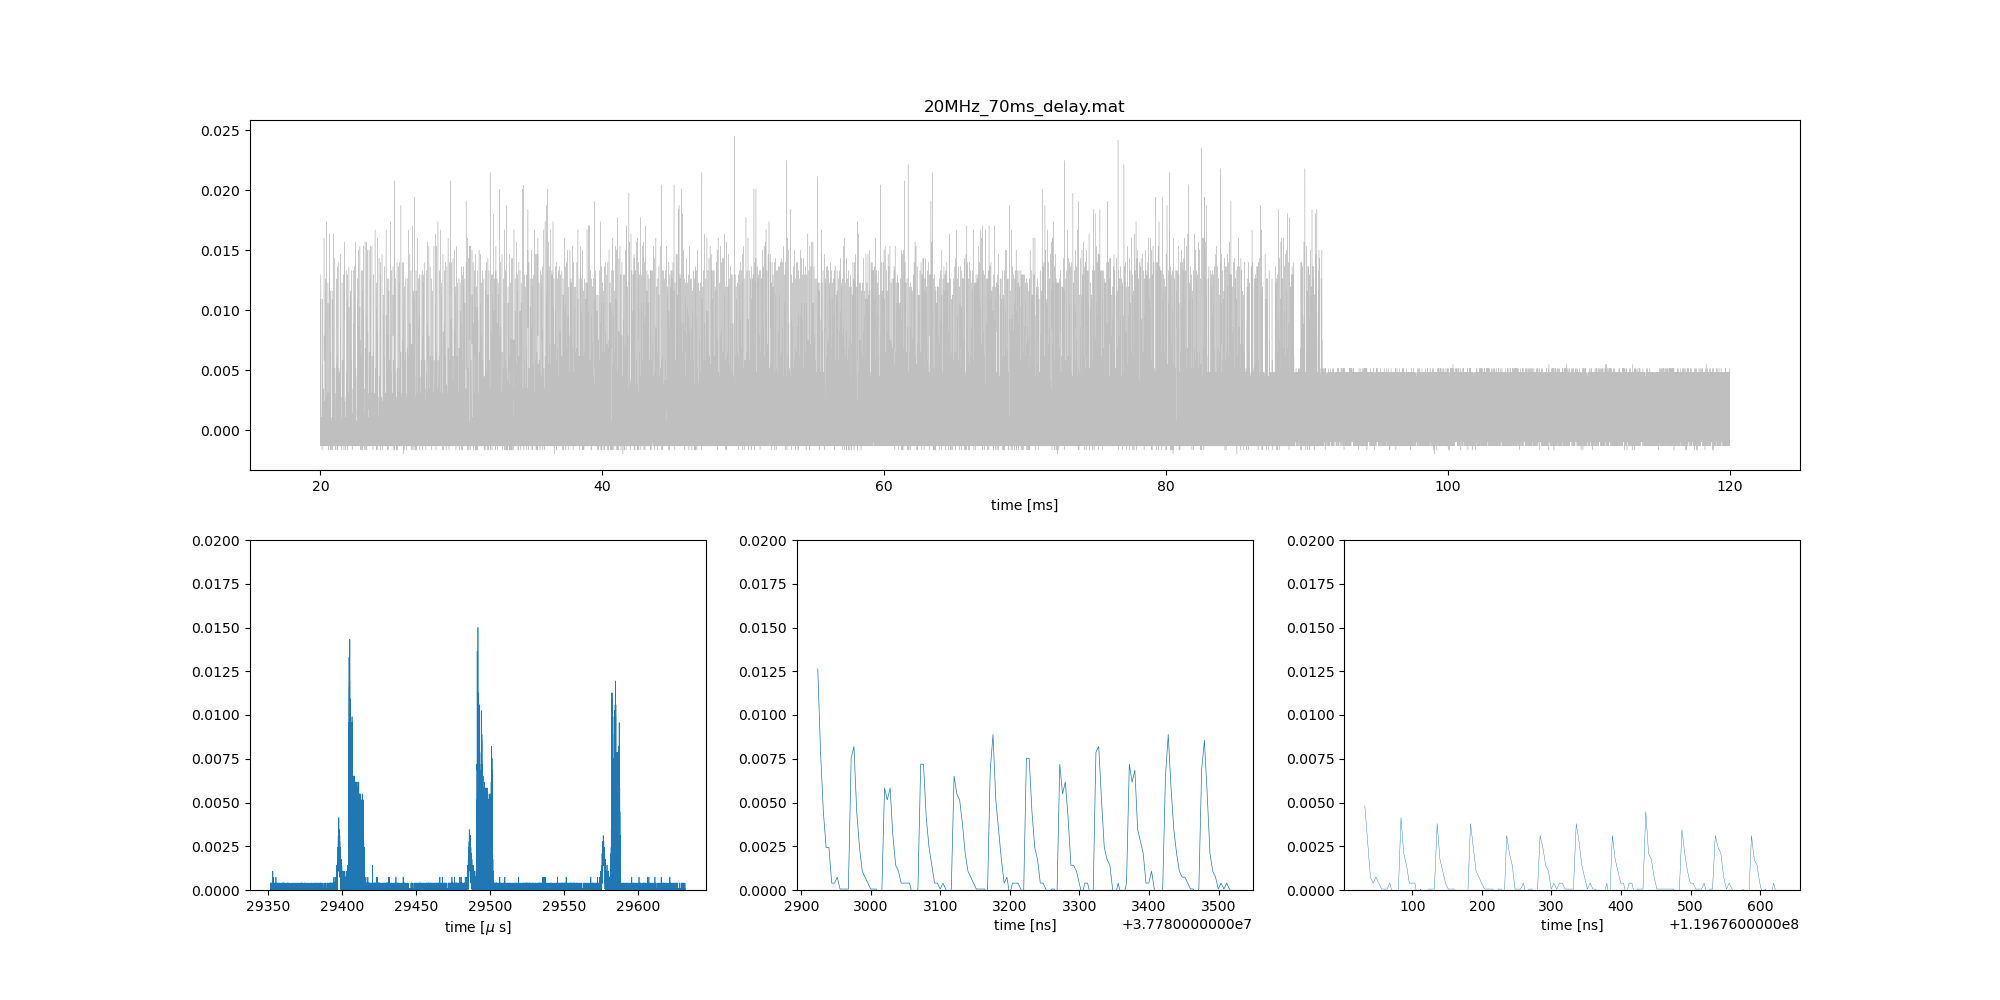
\includegraphics[width=0.79\columnwidth]{Images/Metrics/paper_plot_signals}
	%\caption{ a) Results recorded with reduced bandwidth (20 MHz) detection
		%illustrating the $100$~ms transient regime of Q-switched mode-locked
		%operation before stable mode-locking. The region labeled 'b' \mb{where? Increase size of font and labels!} in the time
		%trace is shown in more detail in panel (b). 
		%The total time record shown corresponds
		%to 2.6 million round trips. b) Results from separate measurements using
		%$30$GHz bandwidth detection, showing how the laser output during the
		%Q-switched mode-locked regime consists of transient bursts of temporal
		%width $10\mu$s separated by $70\mu$s period. The expanded view shows how
		%unstable mode-locked pulses at $50$~ns period are generated under each
		%burst. c) Results using $30$~GHz detection but in the stable mode-locked
		%regime, showing a regular train of pulses with constant intensity. The time axis divisions (div.) are as indicated.}
	\label{fig:Goery_paper}
\end{figure}
a
\begin{figure}
	\centering
	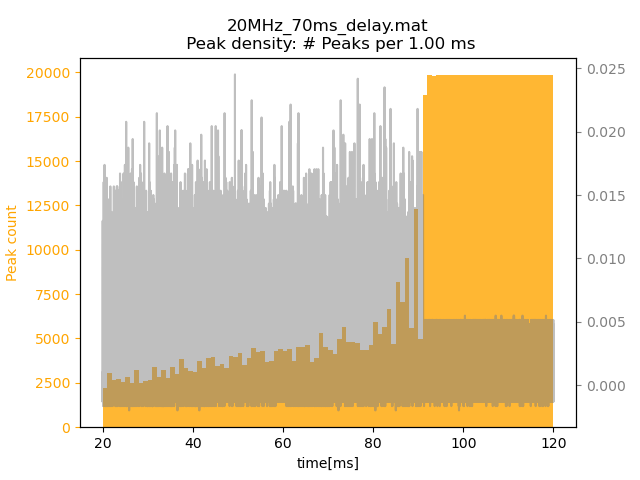
\includegraphics[width=0.4\columnwidth]{Images/Metrics/peak_density}
	\caption{Amount of events per ms. \mb{What is in gray, in yellow? Axis?} }
	\label{fig:Goery_density1}
\end{figure}